\documentclass{../Misc/MontavonLaTeX/Montavon}
\usepackage{wasysym}
\usepackage{multirow}
\usepackage{isotope}
\usepackage[autostyle=true,german=quotes]{csquotes}
\usepackage{mathtools}
\usepackage[biblabel]{cite}
\usepackage[font=small,labelfont=bf]{caption}
\usepackage{svg}

\usepackage{feynmp}
\DeclareGraphicsRule{.1}{mps}{*}{}

\newcommand{\e}[1]{\ensuremath{\times 10^{#1}}}
\newcommand{\defeq}{\vcentcolon=}
\newcommand{\eqdef}{=\vcentcolon}
\newcommand{\gdagzn}{$\textrm{GdAg}_{1-x}\textrm{Zn}_x$}

\graphicspath {{out/}{bilder/}{data/}}
\heads{RWTH Aachen \\ F.-Praktikum}{F12 \\ Magnetische Phasenübergänge}{Jonas Lieb (Gruppe 20)\\ 30. März 2015} 
\date{30. März 2015}

\newcommand{\thirdwidth}{0.32\textwidth}
\newcommand{\halfwidth}{0.48\textwidth}
\newcommand{\fullwidth}{1.0\textwidth}

\setlength\parindent{0pt}
\setlength{\parskip}\medskipamount
\begin{document}

\title{Fortgeschrittenenpraktikum \\ \quad \\ Protokoll zu den Versuchen über \\ Magnetische Phasenübergänge}
\author{Jonas Lieb, 312136 \\ \emph{Gruppe 20} \\ \\  RWTH Aachen}
\maketitle

%\begin{abstract}
%\end{abstract}

\newpage

\setcounter{tocdepth}{2}
\tableofcontents
\newpage

\section{Einleitung}
In diesem Versuch werden die magnetischen Eigenschaften eines Supraleiters und einer \gdagzn-Probe bei verschiedenen Temperaturen untersucht. Um die komplexe magnetische Suszeptibilität $\chi$ zu messen, werden die zu untersuchenden Proben einzeln in ein Hartshorn-Spulensystem eingeführt. Dieses besteht aus einer Primärspule, an der Wechselstrom anliegt, und aus zwei Sekundärspulen, wovon eine die Probe umschließt. Die Spannungsdifferenz der beiden Sekundärspulen wird mit einem Lock-In-Verstärker vermessen. Nach geeigneter Kalibrierung ist das integrierte Ausgangssignal direkt proportional zur Suszeptibilität $\chi$.

Im ersten Versuchsteil werden jedoch zunächst Vorversuche zum Lock-In-Verstärker durchgeführt, die zu einem besseren Verständnis der eingesetzten Messtechnik beitragen sollen.

\section{Vorversuche zum Lock-In-Verstärker}
\subsection{Theorie}
Der Lock-In-Verstärker besteht u.a. aus einem Signalgenerator, einem Verstärker, einer Differenzeinheit, einem Filter, einer Multiplikationseinheit und einem Integrationsteil. 

Der Signalgenerator erzeugt eine Sinus-Schwingung (\emph{Referenzsignal}), welche zum Betreiben des Versuches genutzt wird. Aus den beiden resultierenden Messspannungen wird die Differenz gebildet. Diese wird daraufhin mit einem Hoch-, Tief- oder Bandpass gefiltert und verstärkt. Das verstärkte Signal wird mit dem Referenzsignal multipliziert und über mehrere Perioden integriert. Integrationszeit und relative Phase des Referenzsignales zum Messsignal sind dabei einstellbare Parameter. Das integrierte Signal liegt am Ausgang an und kann mit einem Multimeter oder einem Oszilloskop ausgelesen werden.

\subsection{Der Tiefpass}
\subsubsection{Aufbau und Durchführung}
Der Lock-In-Verstärker wird in diesem Versuchsteil noch nicht betrieben. Stattdessen wird ein Tiefpass 1. Ordnung, bestehend aus einem RC-Glied, aufgebaut. Dabei wird ein Widerstand $R = 1.5 \unit{k\Omega}$ und ein Kondensator $C = 100 \unit{nF}$ in Reihe geschaltet. 
Als Stromquelle $U_e$ wird ein Funktionsgenerator verwendet. Er erzeugt ein Sinus-Signal, dessen Frequenz wird vom 10 bis 21000 $\unit{Hz}$ variiert wird und dessen Effektivspannung des Signals $\approx 1.0 \unit{V}$ beträgt. 
Die Spannung $U_a$ über dem Kondensator wird mit einem Oszilloskop gemessen, dabei wird die Amplitudenspannung vom Oszilloskop berechnet (max-Funktion) und per Hand abgelesen.

\begin{figure}[htbp]
\centering
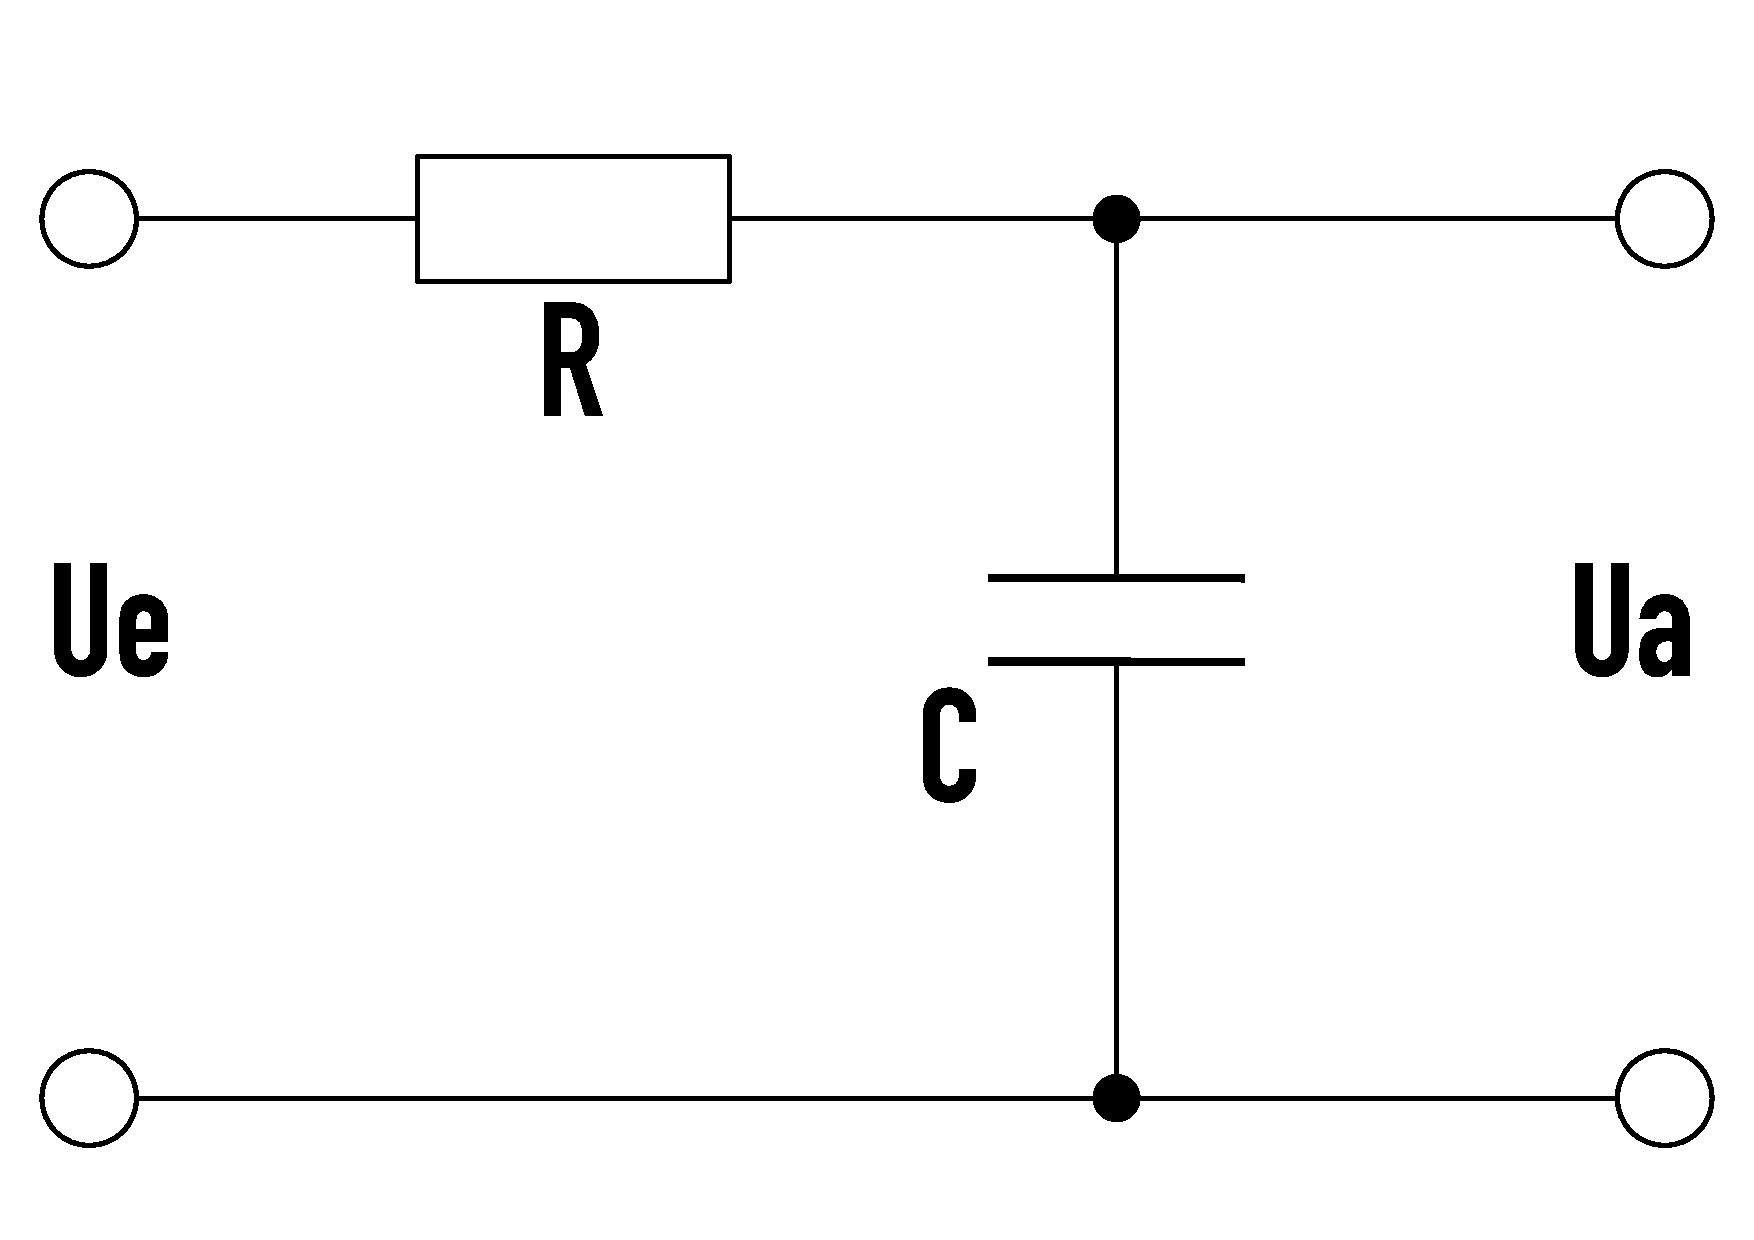
\includegraphics[width=\halfwidth]{schaltung_tiefpass}
\caption{Tiefpass aus einem RC-Glied. Hier verwendet wurden $R \approx 1.5 \unit{k\Omega}$ und $C \approx 100 \unit{nF}$. Bildquelle: public domain.}
\end{figure}

Zur Kontrolle werden Widerstand und Kondensator zunächst mit einem Multimeter vermessen. Dabei ergibt sich der genauere Widerstand von $(1.487 \pm 0.001) \unit{k\Omega}$ und eine Kapazität von $C = (94.5 \pm 0.1) \unit{nF}$. Diese Werte werden im folgenden verwendet. Außerdem wird die Spannung am Kondensator ebenfalls mit dem Multimeter aufgenommen, um die Messergebnisse des Oszilloskops zu überprüfen.

\subsubsection{Rohdaten}
\begin{figure}[htbp]
\centering
\includegraphics[width=\halfwidth]{tiefpass_raw}
\caption{Rohdaten der Vermessung des Tiefpasses. Da mit dem Oszilloskop Amplitudenmesswerte und mit dem Multimeter Effektivwerte gemessen werden, müssen die Oszilloskopspannungen mit $1 / \sqrt{2}$ gewichtet werden, damit sie verglichen werden können.}
\label{fig:tiefpass_raw}
\end{figure}

Die Rohdaten in grafischer Form befinden sich in Abbildung \ref{fig:tiefpass_raw}. Die Oszilloskopspannungen sind Amplitudenwerte, daher um $\sqrt{2}$ höher als die Multimeterwerte.

\subsubsection{Auswertung}
\begin{figure}[htbp]
\centering
\includegraphics[width=\fullwidth]{tiefpass}
\caption{Skalierte Daten der Tiefpassmessung. Eingezeichnet ist außerdem die theoretische Kurve mit $R = 1.487 \unit{k\Omega}$ und $C = 94.5 \unit{nF}$, und die entsprechende Grenzfrequenz $f_g = \frac{1}{2 \pi R C}$ bei $\frac{U_a}{U_e} = \frac{1}{\sqrt{2}}$.}
\label{fig:tiefpass}
\end{figure}
Zur Auswertung werden die Werte zunächst skaliert. Als Eingangsspannung $U_e$ wird dabei der Mittelwert der ersten 10 Messwerte gewählt. Daraufhin werden die Werte durch $U_e$ dividiert, um das Verhältnis zu berechnen. Dies ist in Abbildung \ref{fig:tiefpass} gezeigt. Ebenfalls eingezeichnet ist die theoretische Erwartung
\[
	\frac{U_a}{U_e} = \frac{1}{\sqrt{1 + \left(\omega R C\right)^2}}
\]
Es zeigt sich, dass die Messwerte des Oszilloskops deutlich näher an der Erwartung liegen, da die Multimeter-Werte systematisch zu niedrig sind. 

Dies zeigt sich auch schon in den Mittelwerten der ersten 10 Spannungen,
$\overline{U_\textrm{Oszi}} / \sqrt{2} = 1.50 \unit{V} / \sqrt{2} = 1.06 \unit{V}$, $\overline{U_\textrm{Multi}} = 1.03 \unit{V}$.

Aus diesem Grund wird im folgenden das Oszilloskop zur Spannungsmessung bevorzugt, da es trotz geringerer Auflösung einen absolut besseren Messwert liefert.

Innerhalb der Schwankungen entspricht die gemessene Grenzfrequenz außerdem der erwarteten.

\subsection{Dämpfungsbereich der internen Filter}
\subsubsection{Aufbau und Durchführung}
In diesem zweiten Vorversuch werden die internen Filter des Lock-In-Verstärkers untersucht. Dafür wird der Ausgang des Referenzsignales direkt mit dem Eingang A des Lock-In-Verstärkers verbunden. Die Amplitude des Referenzsignales beträgt $\approx 100 \unit{mV}$, die Frequenz wird zwischen 100 und 8650 $\unit{Hz}$ variiert. Da die Phase auf $0 \unit{\degree}$ eingestellt ist, ist die Ausgangsspannung unabhängig von dessen Frequenz, solange kein Filter eingestellt ist. 

Nacheinander werden nun der Tief-, Hoch- und Bandpass eingestellt, mit einer Filterfrequenz $f_0 = 1000 \unit{Hz}$. Die Güte des Filters wird auf $Q = 1$ belassen. Der Lock-In-Verstärker integriert das Signal über $300 \unit{ms}$.

Die Ausgangsspannung wird erneut mit Oszilloskop und Multimeter vermessen.

\subsubsection{Rohdaten}
\begin{figure}[htbp]
\centerline{\begin{minipage}{1.2\textwidth}
\includegraphics[width=\thirdwidth]{li_tiefpass_raw}
\includegraphics[width=\thirdwidth]{li_hochpass_raw}
\includegraphics[width=\thirdwidth]{li_bandpass_raw}
\end{minipage}}
\caption{Rohdaten der Vermessung der internen Filter. Links: Tiefpass, Mitte: Hochpass. Rechts: Bandpass.}
\label{fig:interne_filter_raw}
\end{figure}

Die Rohdaten sind in Abbildung \ref{fig:interne_filter_raw} gezeichnet. Erneut zeigt sich, dass die Messdaten des Multimeters systematisch niedriger sind als die des Oszilloskops. Aufgrund der Ergebnisse des ersten Vorversuches werden ausschließlich die Oszilloskopwerte weiter betrachtet.

\subsubsection{Auswertung}
Im ersten Schritt kann eine qualitative Beschreibung der Ergebnisse geschehen: wie erwartet passieren beim Tiefpass ausschließlich Frequenzen $f < f_0$, beim Hochpass $f > f_0$ und beim Bandpass $f_1 < f_0 < f_2$, wobei $f_1$ und $f_2$ zwei Grenzfrequenzen sind, die im Anschluss bestimmt werden.
Auffällig ist jedoch, dass anders als beim Tiefpass erster Ordnung, auch negative Spannungswerte angenommen werden. Jenseits von $f_0$ fällt die Spannung dabei von $1.4 \unit{V}$ auf bis zu $-0.4 \unit{V}$ ab und nähert sich dann asymptotisch $0 \unit{V}$ an. In dieser Messung spricht dies für eine Phasenverschiebung des Signals, welche eine negative Spannung am Ausgang des Lock-In-Verstärkers zufolge hätte.
Einzig beim Bandpass bleibt die Spannung im gesamten Messbereich positiv.

Um die Grenzfrequenz zu finden, wird zunächst die vertikale Position $U_a = U_e / \sqrt{2}$ eingezeichnet. Danach kann die Grenzfrequenz und ihr Fehler manuell abgeschätzt werden. Dieser Vorgang ist in den Abbildungen \ref{fig:li_tiefpass} und \ref{fig:li_hochpass} für den Tief- und Hochpassfilter zu sehen. .

\begin{figure}[htbp]
\centering
\includegraphics[width=\fullwidth]{li_tiefpass}
\includegraphics[width=\fullwidth]{li_hochpass}
\caption{Auswertung der internen Filter. Oben: Tiefpass. Es wird eine Grenzfrequenz von $(1273 \pm 20) \unit{Hz}$ bei einer Filterfrequenz von $f_0 = 1000 \unit{Hz}$ abgelesen. Unten: Hochpass. Es wird eine Grenzfrequenz von $(642 \pm 30) \unit{Hz}$ bei einer Filterfrequenz von $f_0 = 1000 \unit{Hz}$ abgelesen.}
\label{fig:li_hochpass}
\end{figure}

Die Grenzfrequenz $f_g$ des Tiefpasses ist deutlich niedriger als $f_0$ und die des Hochpasses deutlich höher. Auffällig ist außerdem, dass $f_0$ anscheinend die Frequenz angibt, ab welcher $U < 0$.

Für den Bandpassfilter kann eine genauere Methode angewendet werden: in erster Näherung kann eine Cauchy-Lorentz-Verteilung 
\[
	f(x) = \frac{1}{\pi} \frac{s}{s^2 + (x-t)^2}
\]
angepasst werden, da dies die erwartete Funktion eines getriebenen Oszillators und eines Bandpassfilters erster Ordnung ist.

\begin{figure}[htbp]
\centering
\includegraphics[width=\halfwidth]{li_bandpass_fit}
\includegraphics[width=\halfwidth]{li_bandpass_residual}
\caption{Auswertung des internen Bandpasses. Es wurde eine Cauchy-Lorentz-Verteilung auf die logarithmierten Daten angepasst. Trotz systematischer Streuung war die Anpassung erfolgreich, da die Genauigkeit besser ist als manuelle Ablesegenauigkeit.}
\label{fig:li_bandpass}
\end{figure}

Diese Anpassung ist in Abbildung \ref{fig:li_bandpass} gezeigt. Obwohl die Daten im Residuengraphen systematisch streuen, was zeigt, dass es sich hierbei nicht um einen Bandpass 1. Ordnung handelt, ist diese Anpassung eine gute Näherung.

\begin{figure}[htbp]
\centering
\includegraphics[width=\fullwidth]{li_bandpass}
\caption{Auswertung des internen Bandpasses. Die angegebenen Frequenzen wurden aus den Fitparametern zurückgerechnet. Die Güte $Q = 1.552 \pm 0.004$ ist deutlich höher als erwartet.}
\label{fig:li_bandpass2}
\end{figure} 

Aus den erhaltenen Parametern $s = (0.2178 \pm 0.0005)$ und $t = (2.9964 \pm 0.007)$ können nun physikalisch relevante Parameter berechnet werden:
Die Peakfrequenz beträgt $f_0 = (991.8 \pm 1.6) \unit{Hz}$, mit einer Spitzenspannung von $(1.461 \pm 0.004) \unit{V}$. Die Bandbreite von $f_1 = (718.2 \pm 1.3) \unit{Hz}$ bis $f_2 = (1369.7 \pm 2.5) \unit{Hz}$ beträgt $B = f_2 - f_1 = (651.5 \pm 2.0) \unit{Hz}$ (siehe auch Abbildung \ref{fig:li_bandpass2}). Dabei wurden die Fehler der Fitparameter mithilfe von gaußscher Fehlerfortpflanzung berechnet. 
Es ergibt sich eine Güte von $Q = f_0 / B = 1.552 \pm 0.004$. Dieser Wert ist deutlich höher als die eingestellte Erwartung von $Q = 1$.

\subsubsection{Ergebnis}
Die internen Filter sind keine Filter erster Ordnung. In der Messung sind negative Spannungen aufgetreten, was für eine Phasenverschiebung des Signals spricht. Außerdem entspricht $f_0$ nicht der Grenzfrequenz, sondern der Frequenz, ab der $U(f) < 0$. Daher sind die Grenzfrequenzen des Tiefpasses niedriger und des Hochpasses tiefer als $f_0$.
Der Bandpass entspricht den Erwartungen insofern, als dass er einen ähnlichen Verlauf wie ein gewöhnlicher Bandpass 1. Ordnung zeigt. Die eingestellte Güte  von $Q = 1$ wird allerdings nicht erreicht, stattdessen beträgt sie $Q = 1.552 \pm 0.004$.

\subsection{Signalfiltern mittels Hoch- und Tiefpass}
\subsubsection{Aufbau und Durchführung}
In diesem Versuch wird die Auswirkung der Filter auf ein Messsignal mit einer  extrinsischen Rauschquelle betrachtet. Dabei wird erneut das Referenzsignal in den Lock-In-Verstärker auf Ausgang B zurückgekoppelt, allerdings gleichzeitig zusätzlich ein Signal mit anderer Frequenz mit Ausgang A verbunden. Dieses Störsignal wird von einem externen Frequenzgenerator erzeugt. 
Mit einem Oszilloskop werden Referenzsignal, Störsignal und das gefilterte, überlagerte Signal beobachtet. Letzteres wird dabei durch den Ausgang \emph{SIG.MON}, also den Signalmonitor dem Oszilloskop zugeführt.

Als Referenzsignal wird $f_R = 3500 \unit{Hz}$ gewählt. Das Störsignal wird mit $f_S = 200 \unit{Hz}$ gewählt. Die Amplitude des niederfrequenten Störsignals beträgt $420 \unit{mV}$, während das Referenzsignal auf $100 \unit{mV}$ gestellt ist.
Die erste Messung enthält keinen Filter, danach werden nacheinander ein Hochpass und ein Tiefpass mit $f_0 = 1000 \unit{Hz}$ angewendet.

\subsubsection{Auswertung}
\begin{figure}[htbp]
\centering
\includegraphics[width=\fullwidth]{F0031TEK}
\includegraphics[width=\halfwidth]{F0032TEK}
\includegraphics[width=\halfwidth]{F0033TEK}
\caption{Demonstration der Filterung eines Störsignales. Oben: kein Filter. Unten links: Hochpassfilter bei $f_0 = 1000 \unit{Hz}$. Unten rechts: Tiefpassfilter bei $f_0 = 1000 \unit{Hz}$. \\Kanal 1 (gelb, Mitte) zeigt das Referenzsignal mit $3.5 \unit{kHz}$. Kanal 2 (grün, unten) zeigt das Störsignal mit $200 \unit{Hz}$, 5-fach verkleinert. Kanal 3 (violett, oben) zeigt das gefilterte, überlagerte Signal.}
\label{fig:filtering}
\end{figure}

Die Daten sind als Oszilloskop-Bildschirmfotos in Abbildung \ref{fig:filtering} zu sehen. Wie erwartet zeigen sich in Kanal 1 und 2 das Referenzsignal mit $3.5 \unit{kHz}$ und das Störsignal mit $200 \unit{Hz}$. Das überlagerte Signal entspricht auch der Erwartung, einer Sinus-Schwingung mit geringer Amplitude, auf einer zweiten Schwingung mit größerer Amplitude und längerer Periode.

Durch Anwenden des Hochpassfilters wird das niederfrequente Signal nahezu vollständig unterdrückt. Da der Hochpassfilter in diesem Bereich sogar negative Spannung erzeugt, ist die niedrige Frequenz leicht invertiert zu erkennen, d.h. dort, wo die grüne Kurve ein Minimum besitzt, besitzt das Störsignal in der Überlagerung ein Maximum.

Auch das Anwenden des Tiefpassfilters ergibt das gewünschte Ergebnis. Die hochfrequente Schwingung ist nicht mehr zu erkennen.

\subsection{Zeitkonstante}
\subsubsection{Aufbau und Durchführung}
In diesem Versuchsteil wird ermittelt, welches Verhältnis zwischen Referenzfrequenz und Integrationszeit im Hauptversuch eingestellt werden kann. 

Dafür wird die Integrationszeit fest auf $10 \unit{ms}$ eingestellt und die Frequenz in Schritten von 50 bis 1000 $\unit{Hz}$ erhöht, während die integrierte Spannung mit dem Oszilloskop abgelesen wird.

Das Referenzsignal wird direkt in Eingang A des Lock-In-Verstärkers eingespeist und die Phase um $\pi / 2$ verschoben, sodass bei optimaler Integrationszeit ein integriertes Signal von $U = 0$ erwartet wird. 
Um die Phase möglichst fein einzustellen, wird daher zunächst eine hohe Frequenz eingestellt und der Betrag der Ausgangsspannung minimiert. Dabei ergibt sich eine Feineinstellung von $88.4 \unit{\degree}$.

Als Fehler auf die Werte wird im Oszilloskop zusätzlich der Peak-To-Peak-Wert abgelesen.

\subsubsection{Auswertung}

\begin{figure}[htbp]
\centering
\includegraphics[width=\fullwidth]{integration_time}
\caption{Messung der Spannung eines $\pi / 2$-phasenverschobenen Signals verschiedener Frequenzen. Mit zunehmender Frequenz nähert sich der Wert dem optimalen Wert bei $U = 0$, da über mehr Perioden integriert wird.}
\label{fig:integration_time}
\end{figure}

Die Daten (Abbildung \ref{fig:integration_time}) zeigen deutlich den erwarteten Verlauf. Mit zunehmender Frequenz wird über mehr Perioden integriert, was zur Folge hat, dass das Integral genauer bei $U = 0$ auskommt. Die Werte bei $50 \unit{Hz}$ sind besonders unsicher, da eine Periode dort $20 \unit{ms}$ dauert, was der doppelten Integrationszeit entspricht. 

\begin{figure}[htbp]
\centering
\includegraphics[width=\halfwidth]{integration_time_log_fit}
\includegraphics[width=\halfwidth]{integration_time_log_residual}
\caption{Anpassung der Daten aus Abbildung \ref{fig:integration_time} in logarithmierter Form an eine Gerade. Auf der horizontalen Achse wurde die Anzahl der Perioden $T \cdot f$ in $T = 10 \unit{ms}$ aufgetragen. Es ergibt sich das Modell $U(n = T\cdot f) = (72.4 \pm 2.7) \unit{mV} \exp\left(-(0.433 \pm 0.008) n\right)$, das im Bereich von 100 bis 700 $\unit{Hz}$ (1-7 Perioden) gilt.}
\label{fig:integration_time_fit}
\end{figure}

Da die Daten exponentiell abfallen zu scheinen, kann eine lineare Regression an die Daten in logarithmierter Form ausprobiert werden. Schränkt man die Daten dabei auf den Bereich von 100 bis 700 $\unit{Hz}$ ein, so gelingt die Anpassung (siehe Abbildung \ref{fig:integration_time_fit}). Daraus ergibt sich ein Model
\[
U(n=T \cdot f) = (72.4 \pm 2.7) \unit{mV} e^{-(0.433 \pm 0.008) n}
\]

\subsubsection{Ergebnis}
Mit den Messungen dieses Versuchsteils wird es gelingen, eine geeignete Integrationszeit und Frequenz für den Hauptversuch zu wählen.

Da der Computer in $333 \unit{ms}$-Intervallen Daten aufzeichnet, empfiehlt es sich, die nächst kleinere Integrationszeit, $300 \unit{ms}$ zu wählen.
Beeinflussende Faktoren bei der Wahl der Frequenz sind nun, dass sie möglichst hoch sein muss, damit die Integration gelingt, jedoch nicht zu hoch, da der Aufbau nicht mit Hochfrequenzbauteilen (z.B. Kabeln) ausgestattet ist. Außerdem sollte die Frequenz kein ganzzahliges Vielfaches der Netzfrequenz von $50 \unit{Hz}$ sein.

Für die folgenden Versuche wird daher eine Frequenz von $970 \unit{Hz}$ gewählt. Dies entspricht 291 Perioden pro Integrationsintervall, sodass der Fehler nach dem Modell aus diesem Versuchsteil in der Größenordnung $< 10^{-55}$ liegt, also vernachlässigbar gegenüber anderen Fehlerquellen wird. 


\section{Hauptversuch}
\subsection{Kalibrierungsmessungen am Supraleiter}
\subsubsection{Berechnung der einzustellenden Empfindlichkeit}

\subsection{Messung der \gdagzn-Probe}


\newpage
\begin{thebibliography}{xxxx}
\bibitem{anleitung} Praktikumsanleitung: Versuch PH: Magnetische Phasenübergänge. URL: \url{http://institut2a.physik.rwth-aachen.de/de/teaching/praktikum/Anleitungen/magPhasen_Anleitung.pdf} [Stand: 12.04.2015]
\end{thebibliography}


\end{document}
